\chapter{Úvod}
Tato bakalářská práce se zabývá problematikou vytvoření dema (intra) s~velikostí omezenou na 64kB s~pomocí knihoven OpenGL a SDL.
Budou zde popsány jednotlivé hlavní problémy, na které je třeba se při programování aplikací s~omezenou velikostí zaměřit a bude zde také navržen způsob jejich řešení.

Původně vznikala dema jako podpisy skupin, pohybujících se v~prostředí warezu (počítačového pirátství).
Tato dema byla velmi rozmanitá, existovala například dema pouze s~textovým výstupem, nebo dema s~omezenou velikostí.
Postupem času se dema vyvíjela až do současné podoby.
Nyní jsou dokonce pořádány soutěže ve vytváření jednotlivých typů dem, například do 4kB, do 64kB, atd., v~nichž programátoři ukazují své programátorské schopnosti a umělecké cítění.
Nejznámější takovou soutěží je nyní zřejmě německá soutěž Breakpoint \cite{breakpoint}.
Dema jsou kromě omezení velikostí ještě omezována množstvím pravidel, například zákazem používání externích knihoven.

Práce je strukturována do kapitol podle jednotlivých oblastí problémů, kterým se programátor při vytváření 64kB dema nevyhne.
Tato struktura byla zvoledna z~důvodu rozsáhlosti a odlišnosti všech součástí dema tak, aby na sebe jednotlivé části logicky navazovaly.
Nejprve se zde budeme zabývat celkovým rozvržením programu a dále pak postupně problematickám modelů, materiálů a textur, hudby, scén a nakonec se podíváme na techniky časování dema.

Jelikož popis veškerých technik použitých v~demu by přesáhl rozsah bakalářské práce, budou zde popsány popsány především ty nejzajímavější techniky a nejčastější problémy, se kterými se při vytváření 64kB dem setkáváme. 


\chapter{Framework}
Jelikož většina dem používá velmi podobné postupy a~myšlenky, mohlo by být zajímavou úlohou vytvořit framework, pomocí něhož by bylo možé jednoduše psát nová dema, aniž by bylo třeba implementovat již nespočetněkrát vytvořené funkce pro ovládání scény, hudby a~podobně.
Z tohoto důvodu byl v této práci vytvářen framework, pomocí kterého pak bylo výsledné demo poměrně snadno vytvořeno.

Ačkoliv omezení velikosti výsledného programu na 64kB se zdá obrovské, je možné vytvořit funkční demo i s~takovým omezením.
Takto velký prostor umožňuje programátorovi, za použití správných technik, vytvořit takřka neomezené scény.
Některé z~těchto technik jsou již ve frameworku implementovány a pokud nejsou, dají se jednoduchým způsobem doplnit podle potřeb vytvářeného dema.

Základní myšlenkou pro vytvoření frameworku bylo vytvořit dvě na sobě nezávislé části programu, z~nichž jedna bude obsahovat data frameworku (\emph{/framework}), která jsou pro každé demo stejná a druhá (\emph{/demo}), ve které budou soubory obsahovat informace specifické pro každé demo, psané pomocí tohoto frameworku.

\section{Rozvržení frameworku}
Framework je rozdělen do \emph{manažerů}, které mají na starost práci s~různými logickými částmi frameworku.
\subsection{Manažer materiálů (materialmanager)}
Hlavním úkolem tohoto manažeru je zabezpečování inicializace materiálů a překlad a nahrávání shaderových programů do grafické karty.
Manažer materiálů rovněž při vykreslování objektů na požádání přepíná materiály, které mají být použity.

Podobně jako většina ostatních manažerů i manažer materiálů obsahuje pole struktur, ve kterém jsou všechny záznamy materiálů.
Pomocí tohoto pole potom ostatní managery mohou vybírat, jaký materiál použít a manažer materiálů jej pak nastaví jako aktuální.

\subsection{Manažer modelů (meshmanager)}
Obsahuje funkce pro práci s~modely, jako je například rozkomprimování modelů z~komprimovaného stavu, vytváření rotačních těles.
Pro výpočet normál objektů je použita metoda Gouraudova stínování \cite{gouraud} a pro výpočet texturovacích souřadnic je použit algoritmus.
Další důležitou částí manažeru modelů je algorimus Catmull-Clark pro zaoblování modelů (viz~\ref{catmull}).

Manažer modelů obsahuje pole struktur obsahující rozkomprimované modely a hlavně ID vertex buffer objektů, ve kterých se modely v~grafické kartě nacházejí.
S~těmito záznamy dále pracuje také manažer scén, který z~nich skládá scény.

\subsection{Manažer hudby (musicmanager)}
Pomocí tohoto manažeru je možné přehrávat hudbu, která je uložena ve strukturách, obsahujících notový záznam, seznam nástrojů, seznam melodií a počet úderů za minutu (BPM).
Manažer hudby umí kromě spuštění a zastavení přehrávání ještě například transponovat melodii, nebo dočasně umlčet přehrávání.
Hudbu lze přehrávat pomocí téměř jakéhokoliv nástroje který je nahrán do programu (viz~Kapitola~\ref{hudba}).

Pro přehrávání je používána knihovna SDL audio.

\subsection{Manažer scén (scenemanager)} \label{scenaKratke}
Tento manažer skládá modely z~manažeru modelů a materiály z~manažeru materiálů do sebe a vytváří tak již hotové modely, které pak přiřazuje do stromů scén jako jednotlivé uzly.
Uzly modelů ale nejsou jediné, které je schopen manažer scény vytvořit.
Dále existují ještě kořenové uzly (root nodes), uzly kamer (camera nodes), uzly křivek (curve nodes) a falešné uzly (dummy nodes).
Nad těmito uzly pak zabezpečuje operace jako rotace, posun, změna měřítka a pro uzly kamer navíc například funkci \emph{lookAt} která nastaví pohled kamery na dané místo, změnu perspektivy a další (viz~Kapitola~\ref{scena}).

Manažer scény také zabezpečuje práci s~Bézierovými křivkami.

\subsection{Manažer sekvencí (sequencemanager)}
Manažer sekvencí se stará se o~běh času a časování všech událostí v~demu. Obsahuje velmi podrobné časové záznamy, ve kterých se poecifikuje, co a kdy se má stát a jak k~tomu má dojít. Pomocí těchto záznamů je možné provést velké množství operací, a tak řídit veškeré dění v~demu.
K~těmto záznamům má uloženy všechny křivky, rotace a šumy, které jsou v~záznamech použity (viz~Kapitola~\ref{sekvence}).

\subsection{Manažer textur (texturemanager)} \label{texturemanager}
Texturový manažer slouží vytváření a používání textur. Požadovanou texturu může vytvořit jako složení více základních textur, přes které navíc může ještě aplikovat různé filtry.
Tímto způsobem se dá dosáhnout velmi různorodých textur. 
Dokáže také například vytvořit normálovou mapu používanou v~bump mappingu (viz~Kapitola~\ref{textury}).

\subsection{Generovací skripty}
Další velmi důležitou součástí frameworku jsou generovací skripty, pomocí nichž se převádějí modely a záznamy hudebních nástrojů do formátu, který je co nejmenší a který je framework schopen zpracovat.
\subsubsection{Skript komprimující modely} \label{scriptRaw2c}
Skript je napsaný ve skriptovacím jazyku Python.
Jeho hlavním úkolem je převést model vytvořený například v~Blenderu z~formátu .raw do zdrojových souborů jazyka C.
Po této konverzi se dají data poměrně jednoduše zkomprimovat (viz~\ref{komprese}).
\subsubsection{Skript ukládající hudební nástroje} \label{scriptInstruments}
I~tento skript je psaný v~jazyce Python, používá však navíc modul \emph{pylab}.
Ze zdrojového souboru \emph{.wav}, který obsahuje příklad jednoho tónu zahraného na požadovaný nástroj, skript vygeneruje zdrojové soubory v~jazyce C.
Takto vygenerované soubory pak obsahují informaci o~zvuku, který nástroj vydává a manažer hudby je schopen takový zvuk přehrát (viz~kapitola~\ref{hudba}).
 

\chapter{Kompilace}
Pro psaní dema byl zvolen jazyk C, z~důvodu jeho nizkoúrovňovosti a dobré možnosti optimalizace.
Pro překlad je používán překladač GCC.
Aby bylo dosaženo co nejmenšho výsledného programu, jsou v~překladači zapnuty přepínače, které sice mají v~některých případech nežádoucí účinky, ale úspora místa nebo zrychlení běhu výsledného programu, které tyto přepínače umožní daleko převáží nevýhody.
\section{Použité přepínače} \label{prepinace }
\subsection{\texttt{-nostdlib, -nodefaultlibs, -nostartfiles}}
Přepínač \texttt{-nostdlib} vypne používání standartních systémových knihoven při linkování programu, takže budou přilinkovány pouze ručně specifikované knihovny.
To zmenší výsledný program o~téměř 5kB, což je pro maximálně 64kB velká dema velmi velká úspora paměti.
Odstranění standartních knihoven ale způsobí, že nebude specifikován vstupní bod programu, nebo že budou chybět důležité funkce, jako například \texttt{exit()}.

Absenci vstupního bodu programu jednoduše vyřešíme přidáním přepínače \texttt{-emain}, který vstupní bod programu nastaví na funkci \texttt{main()}.

Chybějící funkce jako například \texttt{alloc()}, nebo \texttt{realloc()} se dají \uv{nahradit} tím, že se při překladu použije přepínač \texttt{-lgcc}.
Tím se přilinkuje většina důležitých funkcí potřebných k~běhu programu.
Mohlo by se zdát, že to je porušením pravidla o~nepoužívání externích knihoven, ale jelikož tento přepínač zabezpečuje podobné funkce jako ve Windows WinAPI, tak je povolen              .
Ale i s~použitím přepínače \texttt{-lgcc} v~programu budou chybět některé velmi důležité funkce.
Jediným možným řešením je tedy tyto funkce napsat ručně přímo do programu a používat je místo originálních, nacházejících se ve standartních knihovnách.
Způsob psaní takovýchto chybějících funkcí je demonstrován na funkci \texttt{\_exit()};
\begin{lstlisting}
 void _exit(int status){
	__asm__ __volatile__ (
		"movl $1, %%eax;\n\t"
		"movl %0, %%ebx;\n\t"
		"int $0x80;\n\t"
		:"r"(status)
		: "%eax"
	);
	while(1);
}
\end{lstlisting}

\subsection{\texttt{-ffast-math}}
Tento přepínač výrazně zvyšuje rychlost provádění kódu, ale snižuje přesnost výpočtů. 
\subsection{\texttt{-funsafe-loop-optimizations}}
Předpokládá, že indexy používané v~cyklech nepřetečou a že cykly s~netriviálními ukončovacími podmínkami jsou konečné.
To umožňuje kompilátoru použít širší škálu optimalizačních metod a může to urychlit běh programu. 
\subsection{\texttt{-fsingle-precision-constant}}
Chová se k~proměnným s~plovoucí řádovou čárkou jako k~proměnným s~jednoduchou přesností.
Proto stačí dělat méně přesné výpočty a program je rychlejší.
\subsection{\texttt{-fno-stack-check}}
Tímto přepínačem je odstraněna kontrola přetečení zásobníku.
\subsection{\texttt{-fno-keep-inline-functions}}
Nezachovává těla funkcí které jsou překladačem automaticky převedeny na inline.
Tím se zmenší velikost výsledného programu.
\subsection{\texttt{-Os}}
Přepínač \texttt{-Os} optimalizuje zdrojový kód tak, aby výsledný program byl co nejmenší. 
Používá přepínače, které speciálně snižují velikost a navíc přidává přepínače stejné jako v~\texttt{-O2}, jen nepoužije ty, které typicky zvyšují velikost programu.
\subsection{\texttt{-s}}
Tímto přepínačem se odstraní všechny tabulky symbolů a relokační informace ze spustitelného souboru.

\section{Komprese spustitelného souboru}
I~v~případě, že jsou přepínače popsané v~kapitole \ref{prepinace} zapnuty, není možné celé demo zmenšit do potřebné velikosti.
Proto je třeba přistoupit ke kompresi výsledného programu nějakým komprimátorem.
Pro toto demo byl zvolen open source komprimátor \emph{UPX (Ultimate Packer for eXecutables)}.
Díky kompresním algoritmům použitým v~\emph{UPX}, je výsledný soubor dema zmenšen na 43\%, tedy ze 112kB na 49kB.


\chapter{3D modely}\label{3dmodely}
Pro potřeby dema je třeba uchovat ve zdrojovém kódu množství 3D modelů. 
Tyto modely jsou většinou velmi složité a proto je nelze vytvořit podobně, jako například rotační modely, které vzniknou rotací funke kolem osy.

Použití 3D modelů s~sebou nese několik problémů.
Jelikož každý model popisuje přesně nějaký tvar v~prostoru, příliš ztrátovou kompresi nelze použít.
Model by pak byl totiž zdeformovaný.
Nabízejí se tedy dvě řešení -- buď bezztrátová komprese, nebo komprese, která povede ke zmenšení kvality modelu.
Ač se zdá, že druhá možnost je nevhodná, zmenšení kvality modelu nemusí být tak významné, jak by se dalo očekávat.
Existují totiž algoritmy, jako například Catmull-Clark (viz~kapitola~\ref{catmull}), které jsou schopny nízkopolygoniální model zjemnit a zahladit.

3D modely se skládají z~trojúhelníků a čtverců (quadů).
Každý trojúhelník a quad se pak skládá z~vrcholů, což jsou vlastně body v~3D prostoru a indexů, které říkají, jaké vrcholy mají být použity pro vytvoření každého trojúhelníku nebo quadu.

\section {Reprezentace dat a vykreslování}
\subsection {Reprezentace dat}
Z~důvodu šetření velikosti cílového programu jsou z~modelů již při kompresi (pro modely generované uvnitř dema, při vytváření modelu) odstraněny trojúhelníky a jsou nahrazeny tzv. degenerovanými quady.
Díky tomuto kroku je nyní možné všechny operace s~modelem uvniř programu omezit pouze na operace s~quady.

\begin{figure}[h]
    \begin{center}
      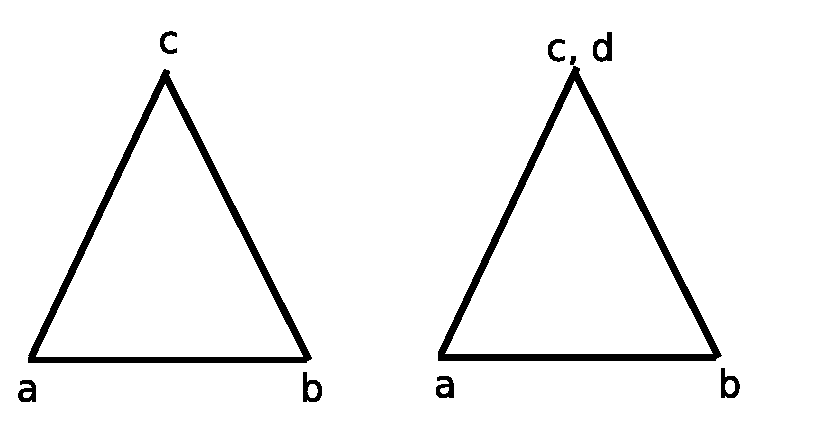
\includegraphics[scale=0.65]{fig/degenQuad} 
      \caption{vlevo -- obyčejný trojúhelník, vpravo -- degenerovaný quad} 
      \label{degQuadFIG}
    \end{center}
\end{figure}

Degenerovaný quad je vlastně trojúhelník, kterému zdvojíme jeden vrchol (viz.~Obrázek~\ref{degQuadFIG}).

Model je v~programu definován strukturou, která obsahuje:
\begin{itemize}
	\item pole vrcholů, z~nichž každý nese informaci o~své pozici v~prostoru, texturových koordinátech a svou normálu
	\item počet vrcholů v~modelu
	\item pole indexů quadů
	\item počet indexů quadů
	\item id vertex bufferu -- nese informaci o~ID bufferu, který obsahuje vrcholy
	\item id index bufferu -- nese informaci o~ID bufferu, který obsahuje indexy jednotlivých quadů
\end{itemize}

\subsection {Vykreslování}
Pro vykreslování byl zvolen nejrychlejší způsob, a to pomocí VBO (Vertex Buffer Object).
VBO vytváří \texttt{buffery}, nacházející se v~paměti grafické karty.
Do těchto bufferů se nahrávaji informace o~vrcholech (3D koordináty, normála, texturové koordináty) a popřípadě i indexech modelů.
Po nahrání všech dat do této výkonné paměti je lze poměrně jednoduše vykreslovat pouhým zvolením aktuálního používaného bufferu.

\section {Komprese modelu} \label{komprese}
Při převádění 3D modelů na data, která budou v~demu uložena, není třeba brát příliš v~potaz časovou náročnost konverze.
Ta se totiž provede pouze jedenkrát, při nahrávání modelu do programu.

Konverze použitá pro převod modelů v~mém demu se skládá z~následujících kroků:

\subsection {Nahrání modelu}
Převádí se model z~formátu \emph{raw}. Zdrojový soubor se nahraje do paměti a rozdělí se na quady a trojúhelníky.
\subsection {Vyčištění modelu}
V~tomto kroku se z~modelu odstraní duplicitní vrcholy, degenerované trojúhelníky (ty se odstraní úplně) a quady (převedou se na trojúhelníky, nebo odstraní).
\subsection {Přeřazení vrcholů}
Přeřazování vrcholů se dělá, protože je třeba najít minimální reprezentaci všech vrchloů
Tento krok obsahuje nejnáročnější operaci s~vrcholy.
Jako první se vyčíslí a uloží všechny možné hrany mezi vrcholy (velmi náročné na výpočetní výkon a paměť).
Tyto hrany jsou převedeny na minimální kostru \cite{minimumSpanningTree}, která je pak posléze převedena na \emph{hamiltonovský cyklus} \cite{hamiltonianPath}.
Převod na hamiltonovský cyklus je ale pouze vhodná heuristika na vyřešení problému.
\subsection {Vygenerování delta souřadnic}
Delta souřadnice jsou souřadnice, pomocí kterých se dá definovat více bodů v~prostoru tak, že se vždy ukládá pouze změna pozice vůdči předchozímu uloženému bodu.
Po převedení minimální kostry na hamiltonovskéhý cyklus je možné odvodit pořadí, v~jakém budou vrcholy ukládány.
Je třeba převést absolutní souřadníce každého vrcholu na delta souřadnice.
Delta souřadnice se počítaji zvlášť v~každé ose, takže ve výsledku vzniknou tři čísla, což jsou absolutní souřadnice prvního bodu a pro každý další vrchol tři čísla ukazující změnu souřadnic v~příslušné ose vůči předchozímu vrcholu.
Delta souřadnicím je pak změněno měřítko tak, aby se dobře ukládaly.
\subsection {Komprese quadů}
V~předchozích krocích se pracovalo pouze s~vrcholy a indexy se pozměnily v~závislosti na změnách vrcholů.
Nyní přistupujeme ke kompresi indexů výsledných quadů.
Doposud se pracovalo jak s~trojúhelníky, tak s~quady.
Aby tedy byla udržena jednotnost polygonů se kterými je pracováno, je třeba převést trojúhelníky na quady.
Komprese quadů funguje na principu vytváření quad stripů. 
Quad stripy jsou způsob ukládání quadů tak, že první quad je uložen celý a každý další pak definují dva nové body a dva poslední body z~předchozího quadu.
Z~toho vyplývá, že čím delší quad stripy se podaří vytvořit, tím více místa bude ušetřeno na ukládání.
Při skládání stripů je také využito toho, že je třeba se zbavit trojúhelníků.
Takže kdykoliv vytvářený quad strip narazí na trojúhelník, vybere se pro degeneraci strana, která umožňuje vytvořit delší strip. 
Podobně se pak pokračuje nad zbylými indexy.
\subsection {Export a použití v~demu}
Výsledný model je exportován do dvojice souborů s~příponou \texttt{.c} a \texttt{.h}.
Ty obsahují delta souřadnice vrcholů, pozici prvního vrcholu, koeficient, kterým je třeba přenásobit delta souřadnice a quad stripy.

V~samotném programu se při nahrávání vezme první vrchol a pomocí delta souřadnic a měřítka se dopočítají zbylé vrcholy.
Quad stripy se opět rozdělí na quady. K~modelu jsou dopočítány normály a texturové koordináty a vrcholy a indexy jsou pak nahrány do grafické karty.

\section {Rotační modely}
Rotační modely vznikají rotováním zadané funkce okolo osy. Tyto modely jsou pro dema výhodné, protože mohou mít velmi vysoká rozlišení a mohou být velmi složité, a přesto je jejich velikost zanedbatelná.
Funkce podle kterých jsou modely generovány jsou zadány jako, jako matematické funkce jazyka C z~$<0,1>$ do $\mathbb{R}^{+}$

\section {Catmull-Clark} \label{catmull}
Jak už bylo zmíněno v~kapitole \ref{3dmodely}, algoritmus Catmull-Clark se používá k~rozdělení plochy na menší časti (quady) a na zjemnění jejího povrchu.
Je to velmi často používaný algoritmus při vytváření dem, protože umožňuje uložení nízkopolygoniálního modelu, což je díky menší potřebě paměti k~uložení modelu velmi výhodné.

\subsection{Popis algoritmu}
Popis práce algoritmu Catmull-Clark \cite{catmullClarkWP}.
Začneme s~libovolným modelem složeným z~polygonů.
Každý vrchol v~tomto modelu nazvěme \emph{původní}.

\begin{itemize}
  \item Pro každý polygon vytvoříme nový \emph{středový vrchol}.
  \begin{itemize}
    \item Pozici středového vrcholu vypočítáme jako aritmetický průměr všech \emph{původních vrcholů} daného polygonu.
  \end{itemize}
  \item Pro každou hranu polygonu vytvoříme nový \emph{hranový vrchol}.
  \begin{itemize}
    \item Pozici hranového vrcholu nastavíme na průměr dvou sousedících \emph{středových vrcholů} a dvou \emph{původních vrcholů}, určujících danou hranu.
  \end{itemize}
  \item Pro každý středový vrchol vytvoříme \emph{hrany} propojující středový vrchol se všemi hranovými vrcholy polygonu.
  \item Pro každý původní vrchol $P$ vypočítáme novou pozici $P'$ jako aritmetický průměr $F$ ze všech $n$ středových vrcholů, náležících polygonům, pro něž je vrchol $P$ jedním z~původních bodů (rovnice \ref{eq1}). Dále vypočítáme aritmetický průměr $R$ ze všech středů hran, které se dotýkají vrcholu $P$. Střed hrany se vypočítá jako aritmetický průměr dvou koncových vrcholů hrany.
\end{itemize}

\begin{eqnarray}
  P' = \frac{F + 2 \cdot R + (n - 3) \cdot P}{n} \label{eq1}
\end{eqnarray}

Algoritmus Catmull-Clark je pro větší modely poměrně pomalý, což ovšem v~demech příliš nevadí, protože veškeré výpočty se mohou provést v~nahrávací sekvenci.
Modelu, na který je Catmull-Clark použit, exponenciálně roste počet polygonů a vrcholů a zabírá mnohem více místa v~paměti, proto by se měl používat v~rozumné míře.

To, jak použití algoritmu Catmull-Clark vypadá, je velmi názorně vidět na obrázku \ref{catmullClarkFIG}.
Oči postavy, které se při přehrávání dema jeví jako kulaté, jsou ve skutečnosti uloženy pouze jako kostky.
Při nahrávání modelu je na kostky dvakrát aplikován algoritmus Catmull-Clark, a tím se původně hranaté oči zakulatily.
Tato metoda je použita na většinu modelů v~demu, s~výjimkou klavíru a židličky, kterým bylo třeba zachovat jejich hranatost.
\begin{figure}[h]
    \begin{center}
      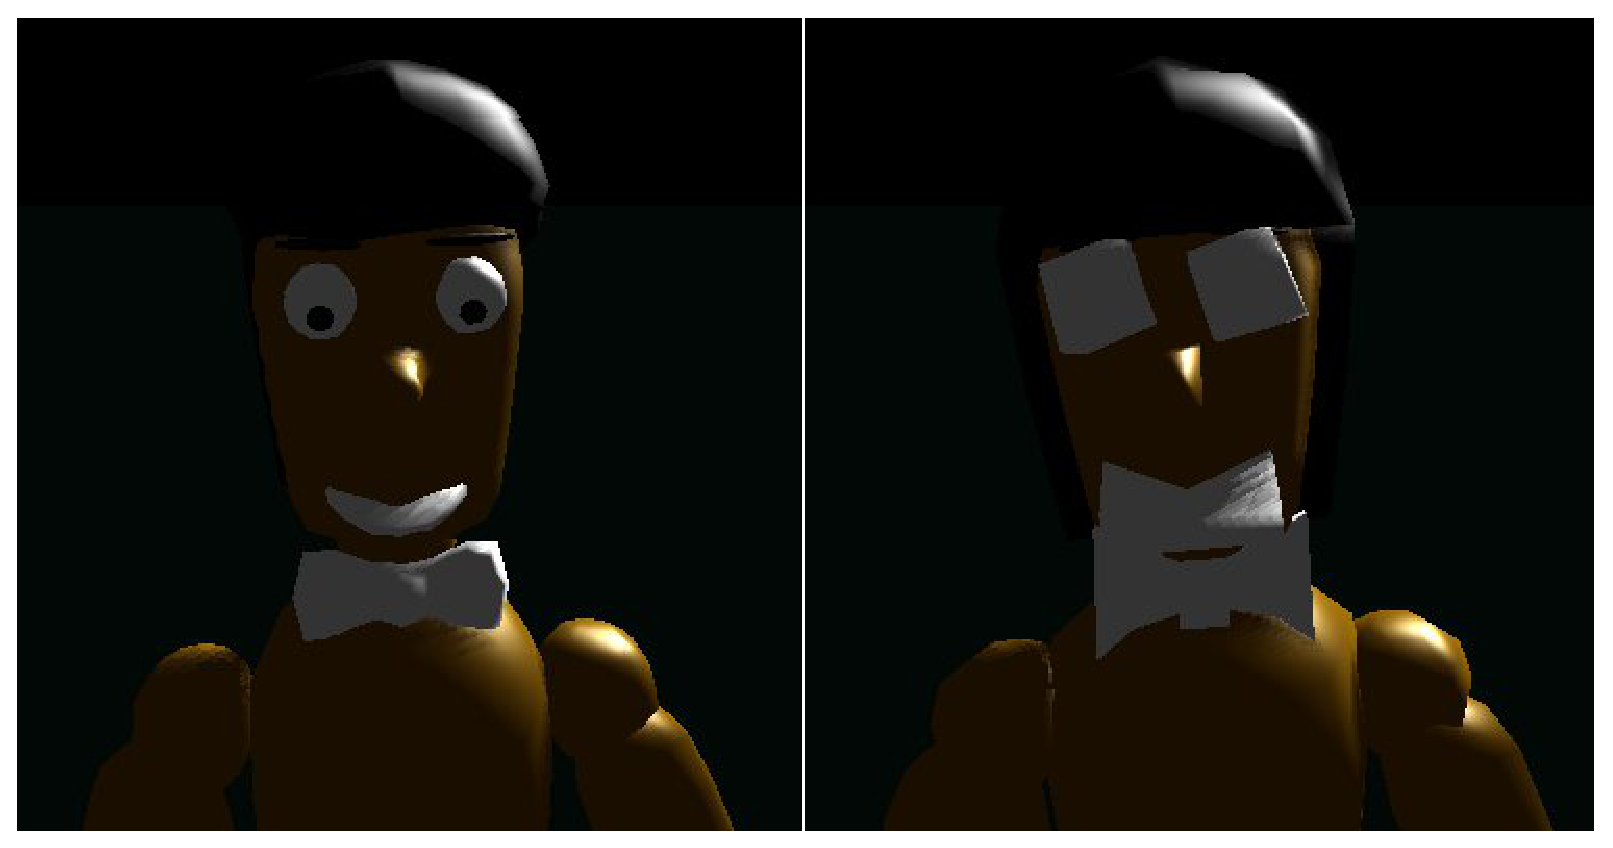
\includegraphics[scale=0.32]{fig/catmullClark} 
      \caption{Model s~a bez použití algoritmu Catmull-Clark} 
      \label{catmullClarkFIG}
    \end{center}
\end{figure}


\chapter{Textury} \label{textury}
O~textury se v~demu stará texturový manažer, který je nejprve při startu programu vygeneruje a potom umožňuje ostatním manažerům, aby s~nimi pracovali.
Pro popis textury je vytvořena speciální struktura ve které jsou zaznamenány všechny potřebné informace o~její výšce, šířce a také samotná data textury, uložená ve formátu RGBA.

Problematika textur je v~demech s~omezenou velikostí poměrně složitá, protože právě kvůli omezené velikosti není možné použité textury ukládat jako obrázky.
Z~toho důvodu se jsou často používány procedurální generátory textur, které požadované textury vygenerují až při   spouštění samotného programu, bez potřeby ukládání velkých obrázků. \cite{texturesCON}
Tento způsob s~sebou ale přináší problém, jak generovat co největší množství rozmanitých textur tak, aby byl generátor co nejmenší a nejefektivnější.

Základní myšlenkou generátoru textur, který je v~tomto frameworku použit, je práce s~vrstvami o~stejné velikosti jako má požadovaná výsledná textura.
Nad těmito vrstvami jsou prováděny jednotlivé operace tak, aby se dosáhlo požadovaného vzhledu výsledné textury.
Tyto operace se dělí do několika skupin.
Pomocí těchto operací se pak typicky vytvoří několik základních (viz~\ref{texturyGen}) vrstev, které jsou pomocí distorzí (viz~\ref{texturyDist}) a operací nad texturami (viz~\ref{texturyOp})  změněny do po požadovanáho vzhledu.
Výsledná textura potom může být ještě obarvena (viz~\ref{texturyBar}), nebo na ni mohou být aplikovány nějaké další speciální efekty (viz~\ref{texturyEfe}).

\section{Generování textur} \label{texturyGen}
Generování textur je prvním krokem pro vytváření textur, pomocí něhož se vytvoří základní vrstvy, na které se pak aplikují různé operace.
Existuje velmi mnoho způsobů jak generovat základní textury.
Zde popíšeme pouze ty, které byly použity v~manažeru textur (viz~\ref{texturemanager}).
\subsection{Sinová plazma}
Sinová plazma je jedním z~nejjednodušších základních efektů \cite{plasma}.
Barva v~libovolném bodě $[X,Y]$ se vypočítá podle vzorce \ref{eq3}, kde $sirka$ a $vyska$ jsou vlastnosti generované textury, $f_x$ a $f_y$ určují frekvenci sinusoid a $off_x$ a $off_y$ definují posunutí v~osách.

\begin{eqnarray}
  hodnota = \frac{sin((x + off_x) \cdot \frac{2 \cdot \pi}{sirka} \cdot f_x) + sin((y + offy) \cdot \frac{2 \cdot \pi}{vyska} \cdot f_y) + 2}{4} \label{eq3}
\end{eqnarray}

\begin{figure}[h]
    \begin{center}
      \includegraphics[scale=0.65]{fig/sineTex} 
      \caption{Sinová plazma} 
      \label{sinTex}
    \end{center}
\end{figure}

\subsection{Osvětlená koule}
Další základní texturou, kterou je možno vytvořit jako počáteční vrstvu, je osvětlená koule (gradient sphere, nebo phong sphere).
Je to velmi jednoduchá textura, ve které se barva bodů určuje podle vzdálenosti od určeného bodu textury.

\begin{figure}[h]
    \begin{center}
      \includegraphics[scale=0.65]{fig/gradTex} 
      \caption{Osvětlená koule} 
      \label{sinTex}
    \end{center}
\end{figure}

\subsection{Value noise a víceoktávový value noise}
Value noise je jedním z~algoritmů, na generování šumu.
Řadí se tak mezi algoritmy jako perlin noise, nebo simplex noise. 
Tyto dva algoritmy nemají oproti value noise při generování dvourozměrných textur, používaných v~tomto frameworku, mnoho výhod a jsou o~dost pomalejší, proto byl zvolen právě value noise.

Algoritmus pro vytvoření value noise je mírně složitější než algoritmy pro vytvoření osvětlené koule a sinové plazmy.
Nejprve se vygeneruje mřížka řídících bodů.
Vzdálenost těchto bodů se vypočítá podle šířky textury a frekvence šumu.
Pro výpočet dalších bodů se používají interpolace z~řídících bodů \cite{noise}.
Pro interpolaci lze použít několik metod, z~nichž v~úvahu připadají tři.
\begin{itemize}
  \item \emph{lineární interpolace}  -- tento druh interpolace generuje v~šumu ostré hrany. Může být použit při generování šumu v~reálném čase, ale pro účely dema není vhodný.
  \item \emph{kubická interpolace} -- použití této metody rozhodně vede k~velmi dobrému výsledku oproti lineární interpolaci. Oproti kosinové metodě je ale výsledek lepší jen minimálně. Obtížnost výpočtu kubické interpolace (interpoluje ze 4 bodů) ji dělá také vcelku nevhodnou k~použití.  
  \item \emph{kosinová interpolace} -- tato metoda je nejlepší z~výše jmenovaných metod. Je rychlá, protože na rozdíl od kubické interpolace počítá pouze se dvěma body a kvalitativní rozdíl výsledků je zanedbatelný.
\end{itemize}

Víceoktávový value noise je vážený průměr šumů s~exponenciálně rostoucími frekvencemi a exponenciálně klesající váhou.
Při jeho generování se zavádí pojem takzvané \emph{výdrže (persistance)}, který určuje, jaký bude pokles amplitudy šumu pro každou oktávu následující po první oktávě.
První oktáva má amplitudu i frekvenci rovné jedné.
Amplituda $a$ a frekvence $f$ každé další $i$-té oktávy se vypočítá podle vzorců \ref{amplpitudaVN} a \ref{frekvenceVN}.
Hodnota víceoktávového šumu $f(x,p)$ se potom vypočítá podle vzorce \ref{multioctaveVN}, kde $x$ je bod pro který se hodnota počítá, $g(x)$ je funkce šumu a $p$ je výdrž.
V~reálu se tato řada nepropočítává do příliš velké hloubky, čím pozdější prvek, tím menší je jeho efekt na výsledek.

\begin{eqnarray}
  a_i & = & a_{i - 1} \cdot vydrz \label{amplpitudaVN} \\ 
  f_i & = & f_{i - 1} \cdot 2 \label{frekvenceVN} \\
  f(x,p) & = & g(x) + p \cdot g(2x) + p^2 \cdot g(4x) + \cdots \label{multioctaveVN}
\end{eqnarray}

Takto generované šumy se dají použít samotné jako univerzální textura, která učiní povrch 3D modelů realističtějším.
Takto byly šumy (Perlin noise) poprvé použity Kenem Perlinem ve filmu Tron.

Šumy však není nutno používat jen na texturování.
V~mém demu se například generují textury šumů, podle kterých se řídí pohyby loutky.
 
\begin{figure}[h]
    \begin{center}
      \includegraphics[scale=0.49]{fig/valueNoiseTex} 
      \includegraphics[scale=0.49]{fig/8octValueNoiseTex} 
      \caption{vlevo -- value noise, vpravo -- osmioktávový value noise} 
      \label{adsrFIG}
    \end{center}
\end{figure}

\section{Operace nad texturami} \label{texturyOp}
Po vytvoření několika vrstev textur a jejich úpravě je možné tyto textury složit do jedné výsledné textury.
To lze provést pomocí operací nad texturami.
Jsou to vlastně matematické operace, které se provedou nad každým pixelem textury.
Ve všech následujících operacích je použita saturační aritmetika s~maximem 1 a minimem 0.
\subsection{Sčítání a odčítání textur}
Při sčítání textur se do výsledné textury pro každý pixel sečtou hodnoty jednotlivých barevných i alfa kanálů sobě odpovídajících pixelů původních textur

U~odčítání textur je použit stejný princip jako u~jejich sčítání.
Hodnoty všech kanálů v~sobě odpovídajících pixelech ležících v~původních texturách se od sebe odečtou a hodnota určující barvu pixelu se uloží do výsledné textury.
\subsection{Násobení a dělení textur}
Operace násobení a dělení textur jsou analogické k~jejich sčítání a odčítání.
\subsection{Negace textury}
Negováním hodnot textury lze dosáhnout velmi pěkně barevných výsledků.
Negace se provádí tak, že pro každý kanál každého pixelu vyjma alfa kanálů, je aktuální hodnota odečtena od maximální hodnoty daného kanálu.
Jsou-li hodnoty v~kanálech uloženy v~intervalu $<0,1>$, pak se výsledná hodnota negace vypočte jako $hodnota = 1.0 - staraHodnota$.

\section{Distorze} \label{texturyDist}
Distorze textur jsou operace, které umí hýbat pixely v~textuře tak, že vytvoří nějaký efekt.
Typickým příkladem distorzní funkce je funkce vytvářející efekt vzhledu mramoru.

\subsection{Sinová distorze}
Sinová distorze je jedna z~nejjednodušších, přesto ale velmi efektní distorzní funkce.
Pro každý pixel v~textuře se vezme hodnota jeho sinu a podle ní se vypočítá pozice, kam se daný pixel přesune.
Jak tato distorze funguje lze velmi pěkně vidět na obrázku \ref{SinDistortFIG}.

\begin{figure}[h]
    \begin{center}
      \includegraphics[scale=0.65]{fig/noSinDistort}
      \includegraphics[scale=0.65]{fig/SinDistort} 
      \caption{vlevo -- původní šum, vpravo -- použita sinová distorze v~ose X} 
      \label{SinDistortFIG}
    \end{center}
\end{figure}

\subsection{Mramor}
Tato distorzní funkce má za úkol vytvořit texturu podobnou mramoru. 
K~jejímu vytvoření je třeba implementovat nějakou funkci, generující víceoktávový šum, například perlin noise, nebo v~našem případě value noise.
V~závislosti na absolutní hodnotě vygenerovaného šumu se pro každý bod textury posune jeho hodnota na jiné místo.

Díky možnosti upravovat různé proměnné při vytváření takovéto textury, například míru rozptylování původní textury šumem, nebo velikost frekvence rozptylu, lze jednoduše vytvořit zajímavé textury, vypadající jako téměř jakýkoliv druh mramoru.

\begin{figure}[h]
    \begin{center}
      \includegraphics[scale=0.65]{fig/marble}
      \caption{Vygenerovaná textura mramoru} 
      \label{MarbleFIG}
    \end{center}
\end{figure}

\section{Barevné operace} \label{texturyBar}
Generované textury jsou vytvářeny jako černobílé.
Pokud má cílová textura mít nějakou barvu, musí být použita funkce na obarvení.
Pro obarvení je pak třeba zadat dvě barvy, na které se bude výsledná textura přebarvovat.
Jedna ze zadaných barev bude nahrazena za černou barvu a druhá za bílou. 
Pokud textura obsahuje odstíny šedi, pak se mezi zadanými barvami lineárně interpoluje výsledná hodnota barvy.

\section{Další úpravy a efekty} \label{texturyEfe}
Existuje obrovské množství dalších operací, které se dají použít pro generování textur.
Výše popsané operace jsou ale již vcelku dostačující k~tomu, aby se daly vytvořit použitelné a pěkné textury.
Další možné operace a efekty pro generování textur lze nalézt na stránkách skupiny Conspiracy \cite{texturesCON}.


\chapter{Materiály a shadery}
Problematika materiálů a shaderů je v~demu řešena pomocí takzvaného materiálového manažeru.
Jeho hlavním úkolem je ukládat informace o~vlastnostech všech materiálů použitých v~demu.
Materiálový manažer je velmi úzce spjat s~texturovým manažerem, od kterého získává potřebné textury.
Tyto textury se přidávají k~materiálu a před vykreslováním modelu se nastaví potřebný materiál jako aktuální.
To nastaví optické vlastnosti materiálu, jako například lesklost nebo barvy odlesků a také nastaví v~grafické kartě, jaký shader bude použit.
Jakmile je materiál nastaven a grafická karta používá příslušný shader, je možné model vykreslit.

\section{Shadery}
Shadery jsou programy určené ke zpracování přímo na grafické kartě.
Jazyků pro psaní shaderů existuje nespočet.
Protože se v~této bakalářské práci zabýváme programováním dem s~použitím knihovny OpenGL, jsou shadery použité pro vytvoření dema psány v~jazyce \emph{GLSL} \cite{OpenGL}.
Tyto shaderové programy jsou pak nahrávány do grafické karty pomocí \emph{OpenGL rozšíření (extensions)} \cite{extensionsOpenGL}.

Jelikož by při vytváření dema s~omezenou velikostí neměly být používány žádné externí knihovny až na několik povolených, jako jsou SDL knihovna, nebo OpenGL, nastává problém, jak inicializovat rozšíření OpenGL, aniž by byla použita knihovna \emph{GLEW (GL Wrengler Library)}, která má mimo jiné na starosti právě nahrávání shaderů.
Jediným řešením je tedy inicializovat rozšíření k~používání ručně.
To se provede v~Unixu pomocí funkce \emph{glXGetProcAddress()}, nebo pomocí funkce \emph{wglGetProcAddress} ve Windows.
Tyto funkce umožní používat rezšíření, aniž by bylo třeba využít nepovolených knihoven.

\subsection{Shadery v~demu}
\begin{figure}[h]
    \begin{center}
      \includegraphics[scale=0.45]{fig/svetloGLSL}
      \caption{Bodové světlo} 
      \label{svetloGlslFIG}
    \end{center}
\end{figure}

Shadery vytvořené pro demo fungují na principu Phongova osvětlovacího modelu a  mají za úkol vypočítat hodnoty osvětlení na scéně v~zavislosti na stínech a pozicích světla a kamery. 
Scéna je osvětlována bodovým světlem s~vlastnostmi pozice, směr, barva a šířka světelného kuželu.

Do programu shaderu jsou nahrávány informace o~scéně (barva vykreslovaného objektu a jeho další vlastnosti, pozice světla, atd.) a mapa stínů, pomocí nichž se vypočítává výsledná barva bodu v~obraze.
Bodové světlo vyzařuje kužel paprsků (viz~Obrázek~\ref{svetloGlslFIG}).

Pro výpočet skutečnosti, jestli je bod osvětlen je třeba nejprve zjistit, zda se nachází paprsek dopadající na bod ve scéně v~kuželu světla.
K~tomu, abychom mohli zjistit, leží-li objekt uvnitř kuželu nám stačí porovnat, je-li úhel $a$ menší, než úhel $b$.
Pokud jsou vektory $smerPaprsku$ a $smerSvetla$ normalizované, pak platí:

\begin{eqnarray}
  smerPaprsku \bullet smerSvetla & = & |smerPaprsku| \cdot |smerSvetla| \cdot cos(a) \\
  smerPaprsku \bullet smerSvetla & = & cos(a)
\end{eqnarray}

Pak tedy můžeme skalární součin vektoru světla ($smerSvetla$) a vektoru právě dopadajícího paprsku ($smerPaprsku$) porovnat s~kosinem úhlu určujícího šířku světelného kuželu ($b$).
Jestliže tedy platí, že $dot(smerSvetla, smerPaprsku) > cos(b)$, pak bod leží na osvětlené části modelu. 

Pokud se bod nenachází v~osvětleném kuželu, bude mu nastavena výsledná barva pouze podle ambientního světla scény a vlastností materiálu, ze kterého je vytvořen model, kterému daný bod patří.
Jestliže se ovšem v~kuželu nachází, pak je třeba dopočítat několik informací -- nachází-li se právě počítaný bod ve stínu vrženém jiným objektem, má-li bod na sobě přímý odlesk od světla, nebo je-li pouze osvětlen difuzním světlem.

\subsubsection{Stíny}
Stíny jsou velmi důležitou součástí scény, protože nejen že přidávají na realističnosti celého dema, ale také pomáhají člověku, který se na demo dívá, jednodušeji poznat polohu modelů ve scéně.

Technika používaná v~demu se nazývá shadowmapping.
Při vykreslování stínů pomocí této techniky je třeba pro každý zdroj světla ve scéně vytvořit texturu, do které se bude vykreslovat hloubková mapa scény z~pohledu světla.
Pro vykreslování scény z~pohledu světla se používají co nejjednodušší shadery, aby se co nejvíce zrychlil proces vytváření potřebných textur.
Pro větší počet světel potom mohou nastávat problémy s~rychlostí programu.
Všechny textury obsahující scénu z~pohledu světel se potom společně s~vektory určující orientaci textur v~prostoru odešlou do shaderu, který je schopen z~nich vypočítat, zda se objekt nachází ve stínu, nebo ne.

Díky tomu, že shader nyní zná hloubku scény z~pohledu světla a z~pohledu kamery, je schopen vypočítat, zda je plocha osvětlená, nebo ne.
Aby hloubková mapa nemusela být vykreslována s~příliš velkým rozlišením, což by sice vytvořilo hladké stíny bez různých artefaktů, ale současně by se velmi zpomalil výpočet hloubkových map, je použito umělé rozmazání stínů.
Tato technika je poměrně nenáročná, s~její pomocí lze s~dobrým výsledkem vytvořit estetický stín bez nevzhledných zubů.
Funguje tak, že pro každý bod, pro který se stín zišťuje, se shader podívá na stíny bodů v~osmiokolí a vypočítá z~nich průměrnou hodnotu stínu.
Hodnota udávající míru zastíněnosti se vždy pohybuje mezi hodnotami od $0$ do $1$ včetně.
Na konci shaderu je touto hodnotou přenásobena barva bodu vypočítaná v~průběhu shaderu.
K~této barvě se úplně nakonec přičte hodnota ambientního světla.

\subsubsection{Přímé odlesky}
Tento efekt lze velmi často vidět na leských předmětech osvětlených silným světlem.
Je to velmi malý, jasně osvětlený bod, vznikající přímým odrazem paprsků od povrchu předmětu k~pozorovateli -- je závislý jak na poloze světla, tak na poloze pozorovatele.
Hodnota přímého odlesku pro každý bod se vypočítá pomocí odchylky normály pixelu a směrového vektoru světla a vlastnosti materiálu zvané odrazivost (shininess). 

\subsubsection{Difuzní světlo}
Difuzní světlo přichází z~velmi vzdáleného zdroje (jako například slunce) a jeho síla se vypočítá v~závislosti na odchýlení normály plochy od směru dopadajícího světla.
Světlo se ještě odráží, ale po odrazu mají všechny paprsky již stejnou intenzitu.

\chapter{Hudba} \label{hudba}
Při vytváření dema s~limitovanou velikostí musí být zvolen takový typ zvukového záznamu, aby nezabral většinu velikosti výsledného programu.
Z~toho důvodu nelze použít klasické hudební soubory jako \emph{.wav}, \emph{.mp3}, nebo \emph{.ogg}. 

Přesto existuje několik možností, jak uložit a přehrávat hudbu v~takto omezeném prostoru.

Nejznámějším způsobem, který lze použít, je \emph{MIDI syntetizátor}.
Je to velmi starý způsob přehrávání hudby, který se používal například i na prvních elektronických hudebních nástrojích.
Hlavní výhodou přehrávání hudby pomocí MIDI je, že program nemusí obsahovat žádný přehrávač, protože o~přehrávání se stará zvuková karta.
Jeho nevýhodou je ale velmi umělý zvuk, který se nedá nijak měnit.
Tento způsob se již téměř nepoužívá, protože nevýhody jeho používání převažují výhody. 
Výjimkou jsou pouze velmi malá dema, např. do 4kB, ale i tam jsou mnohdy spíše používány softwarové syntetizátory.

Dalším způsobem, který lze pro přehrání hudby v~demech používat, jsou \emph{hudební moduly}, mezi něž patří například MiniFMOD.
Největší nevýhodou hudebních modulů je to, že ačkoliv přehrávač nemusí být příliš velký, soubory nesoucí informace o~hudbě zpravidla velké jsou, protože kromě samotné hudby v~sobě ještě nesou informace o~nástrojích.
Názory na ně se na demoscéně různí, nicméně jejich použití není úplně nejčistším řešením, už kvůli větším nárokům na paměť při ukládání hudby. 

Třetím a zřejmě tím nejlepším způsobem je \emph{softwarový syntetizátor}.
Tato metoda zabírá nejméně místa a výsledný zvuk může být poměrně dobrý v~závislosti na způsobu imitace nástrojů, ale notový záznam je vcelku složitý.
V~demoscéně je to nejčastěji používaná metoda především kvůli její malé náročnosti na paměť a velkým možnostem zvuku, proto byla vybrána i pro tento projekt.

\section{Softwarový syntetizátor}
Největším problémem při tvorbě softwarového syntetizátoru bylo navržení způsobu záznamu hudby tak, aby byl co nejpřehlednější a co nejjednodušší.
Nakonec byla pro hudbu vytvořena struktura, která obsahuje informace o~rychlosti hudby a ukazatele na struktury vzorků a stop.
Stopy nesou informaci o~posloupnosti jednotlivých vzorků a mohou být buď nekonečné (opakující se), nebo ukončené po jednom přehrátí.
Vzorky jsou notové záznamy o~délce 16ti not. 

V~softwarovém syntetizátoru používaném v~tomto frameworku jsou nástroje generovány pomocí aditivní syntézy.
Je to způsob generování zvuku pomocí skládání množství harmonických a neharmonických vln (sinusoid) s~rozdílnými frekvencemi a amplitudami.

Při přehrávání se postupuje přes jednotlivé vzorky v~závislosti na informacích ve stopách.
Pro každou notu, která se má zahrát, se zavolá callback funkce daného nástroje, vracející hodnotu signálu nástroje pro daný okamžik a tón.
Tato hodnota  je pak ještě upravena podle aktuální pozice v~ADSR obálce (viz~\ref{ADSR}).

Další problém nastává, když tón, který hraje, má delší trvání, než je interval mezi jednotlivými tóny ve vzorku.
Kvůli tomuto problému v~syntetizátoru existuje buffer právě hrajících tónů, který obsahuje doznívající tóny a zabraňuje nepříjemnému lupání reproduktorů.

\subsection{Převod a nahrávání nástrojů} \label{scriptInstruments}
Vzhledem k~tomu, že syntetizátor funguje na principu aditivní syntézy, můžeme vytvořit informaci o~nástroji ze zvukového souboru obsahujícího příklad zahraného tónu na požadovaný nástroj.
Pro správnou funkčnost skriptu je třeba nainstalovat tři moduly pythonu -- \emph{scilab}, \emph{pylab} a \emph{scikits.audiolab}.

\subsubsection{Postup převodu} \label{prevodInstruments}
\begin{enumerate}
  \item Načte se \emph{.wav} soubor s~nahrávkou požadovaného nástroje. Soubor smí být pouze jednokanálový.
  \item Na nahraný vzorek se použije Fourrierova transformace.
  \item Vytvoří se dvojice frekvence a jí odpovídající hlasitosti.
  \item Změní se frekvence vzorku na $1Hz$, takže nejhlasitější frekvence má hodnotu 1Hz. Tato transformace se provádí, aby se vzorek později dal bez složitějších výpočtů použít na jakýkoliv tón.
  \item Ze všech vzorků je vybráno několik nejhlasitějších frekvencí a ty jsou exportovány do zdrojových souborů jazyka C, tak, aby je framework byl schopen použít.
\end{enumerate}

\subsubsection{Nahrávání nástrojů}
Výstupem převodu vzorku hudebního nástroje na zdrojové soubory je pole dvojic frekvencí a hlasitostí (viz~\ref{prevodInstruments}).
Pomocí tohoto pole se dále vypočítává tvar vlny zvuku požadovaného nástroje při $1Hz$ .
Hodnota vlny nástroje v~čase $t$ při $1Hz$ se z~$n$ těchto dvojic vypočítá podle vzorce \ref{eq2}, kde $f_{i}$ je frekvence a $h_{i}$ je hlasitost $i$-té dvojice.

\begin{eqnarray}
   \sum_{i = 0}^{n} h_{i} \cdot sin(f_i \cdot 2\pi \cdot t)\label{eq2}
\end{eqnarray}

\subsection{ADSR obálka} \label{ADSR}
ADSR obálka je metoda, která umožňuje syntetizátorům generovat reálněji znějící zvuky pomocí měnění amplitudy znějícího tónu v~průběhu času, podobně jako je to u~reálných nástrojů.
ADSR obálka se skládá ze 4 fází -- Attack, Decay, Sustain a Release.

\begin{itemize}
 \item \emph{Attack} -- počáteční fáze, kdy amplituda během krátké doby vystoupá na první úroveň. Například rychlým náběhem na maximální úroveň amplitudy se dají snadno simulovat perkusní nástroje.
 \item \emph{Decay} -- v~této fázi obálka dojde na druhou hodnotu amplitudy. Tato amplituda nemusí být vždy nižší, než amplituda předchozí fáze, ale u~většiny nástrojů tomu tak je.
 \item \emph{Sustain} -- fáze sustain simuluje držení tónu. Ve většině syntetizátorů se k~této fázi přidává ještě informace \emph{hold}, která určuje, jak dlouho se bude amplituda fáze \emph{sustain} držet. Tato hodnota je závislá na typu nástroje, ladění, ale i na délce struny, kterou má simulovat.
 \item \emph{Release} -- poslední fáze, která simuluje například u~klavíru puštění klávesy. Amplituda zvuku postupně klesá na nulovou úroveň.
\end{itemize}

\begin{figure}[h]
    \begin{center}
      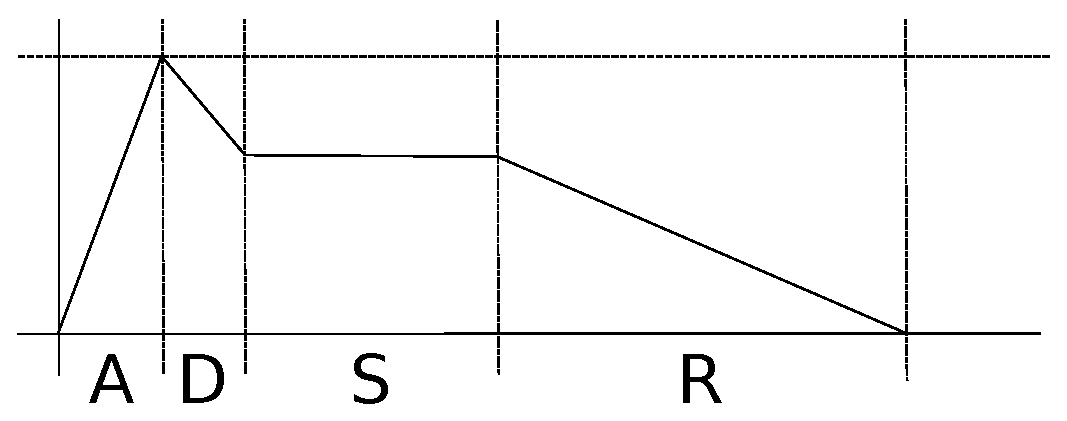
\includegraphics[scale=0.65]{fig/adsr} 
      \caption{ADSR obálka} 
      \label{adsrFIG}
    \end{center}
\end{figure}


\chapter{Scéna} \label{scena}
Scéna je v~demu popisována a ovládána v~manažeru scény, který definuje všechna specifika použitých modelů a dalších objektů použitých ve scéně.

Definuje tedy tvary modelů (převzatých z~manažeru modelů) a nastavuje vlastnosti materiálů (převzatých z~manažeru materiálů), které pro vykreslení objektů budou použity.
Jak již bylo řečeno výše v~kapitole (\ref{scenaKratke}), do scény je kromě modelů možné vložit další objekty, jako například kamery nebo křivky.
O~tyto objekty se také stará manažer scény -- umí je vytvářet, nastavovat atd.
V~neposlední řadě se manažer scény stará o~rotace a posouvání modelů v~prostoru.

Každá scéna je sestavena do stromu. 
Všechny uzly, ze kterých se skládají stromy scén, obsahují svou transformační matici.
Ta je pro každý uzel implicitně nastavena na nulovou matici s~jedničkami na hlavní diagonále (základní pozice těles bez rotací či posunů).
Všechny uzly rovněž obsahují ukazatele na uzly potomků.
Tyto ukazatele určují, jaké další uzly jsou na nich závislé.
Závislé uzly dědí transformace od svých rodičovských uzlů a jejich vlastní transformace jsou pak přidávány k~rodičovským.

Každý strom scény musí začínat kořenovým uzlem, který obsahuje informace o~světle a aktuálně používané kameře.
Jedna scéna může obsahovat i více vnořených kořenových uzlů (scén).
Tyto vnořené scény je potom možné vykreslovat samostatně pouhým zavoláním vykreslování na příslušný kořenový uzel.
Jestliže se narazí na kořenový uzel vnořené scény, pak je tento uzel ignorován a pokračuje se ve vykreslování.

Manažer scény se rovněž stará o~všechny křivky v~demu.
Umožňuje je generovat a vypočítávat aktuální pozici na křivce v~čase.

\section{Kamera}
Aby bylo možné pozorovat scénu, je třeba vytvořit objekt kamery, kterou je možné snímat scénu.
V~jedné scéně se může nacházet více kamer, mezi nimiž je možné přepínat.

Kvůli používání kamery bylo do dema implementováno několik funkcí.
Tyto funkce jsou většinou analogické k~již existujícím funkcím v~některých knihovnách, ale jelikož v~demu se pracuje s~transformačními maticemi zvlášť pro každý model, bylo třeba vytvořit tyto funkce vlastní.

První z~těchto důležitých funkcí nastavuje pozici a směr kamery.
Ze zadaných bodů pozice kamery a cíle, kam se má kamera dívat, a vektoru určujícího směr vzhůru je automaticky nastavena transformační matice kamery podle těchto vstupů.
Druhá funkce nastavuje projekční matici, která definuje přední a zadní ořezové roviny a šířku záběru kamery.

\section{Bézierovy křivky}
Velmi důležitou součástí dema jsou Bézierovy křivky, pomocí michž jsou v~demu uskutečňovány všechny pohyby.
Bézierovy křivky jsou určeny minimálně dvěma body a jejich maximální počet není stanoven.
Jsou-li Bézierovy křivky určeny pouze dvěma body, pak je jejich výsledkem úsečka. 
Jestliže je řídících bodů více a neleží v~přímce za sebou, pak v~závislosti na nich mění svůj směr. 

Křivky jsou vkládány jako součásti scény, což umožňuje hýbat jinak statickými objekty.
Křivky je možné použít i pro definování pozice a pohyu kamery a rovněž pro určování směru jejího pohledu.
Aktuální pozice na křivce v~čase je počítána algoritmem De Casteljau.

\subsection{Algoritmus De Casteljau}
Jde o~algoritmus pomocí něhož se vypočítává pozice v~libovolném čase na Bézierově křivce.
Základním principem tohoto algoritmu je postupné dělení úseček spojujících za sebou jdoucí řídící body obecné Bézierovy křivky.
Ke zjištění pozice bodu na Bézierově křivce v~čase $t$ v~intervalu $<0,1>$ se úsečky spojující řídící body dělí v~poměru  $t : 1 -t$.
Z~každé úsečky takto vznikne právě jeden bod.
Tyto nově vzniklé body se v~dalším kroku opět spojí a dělí se podobně jako v~předchozím kroku.
Nakonec vždy zůstane pouze jediný výsledný bod (bod $D1$ viz~obrázek~\ref{deCasteljauFIG}).

\begin{figure}[h]
    \begin{center}
      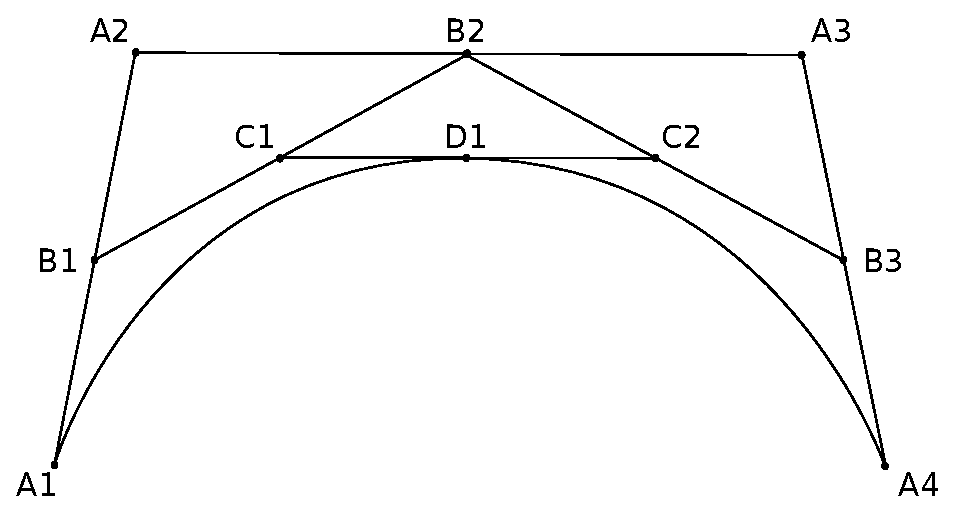
\includegraphics[scale=0.65]{fig/deCasteljau} 
      \caption{Ukázka postupu při algoritmu De Casteljau} 
      \label{deCasteljauFIG}
    \end{center}
\end{figure}

\chapter{Sekvence} \label{sekvence}
Sekvence je nejdůležitější částí dema, která umožňuje řídit veškeré dění v~demu a hlídá uběhlý a zbývající čas.
Je rozdělena do částí dema a frameworku (sekvenční manažer).
Ve frameworku jsou definovány obecné operace, které v~demu bývají velmi často prováděny, jako například rotace modelu v~čase, výměna křivek atd. 
V~části určené pro specifická dema mohou být definovány další operace a nachází se tam hlavní struktura událostí.

Čas je měřen v~milisekundách od zapnutí dema pomocí knihovny SDL a před každým snímkem je aktualizován.
Kromě měření času skevenční manažer provádí různé operace na něm závislé (např. měření počtu snímků za vteřinu).

\section{Část frameworku}
Tato část obsahuje velké množství základních operací se scénou, které s~velkou pravděpodobností programátor při vytváření dema využije.
Není samozřejmě omezen pouze na soubor těchto předdefinovaných funkcí, ale může si sám vytvořit nové funkce v~časti pro demo,

Operace které jsou zde implementováy jsou 
\begin{itemize}
  \item Operace s~hudbou
    \begin{itemize}
     \item Lze za jejich pomocí spouštět, přepínat nebo vypínat hudbu v~přesně daný čas.
    \end{itemize}
  \item Rotace v~čase
    \begin{itemize}
     \item Umožňuje rotovat objekt po nějakou dobu trvání.
     \item Zadává se pouze počáteční a konečný čas a úhel určující o~kolik je třeba model rotovat. 
    \end{itemize}
  \item Posun v~čase
    \begin{itemize}
     \item Umožňuje pohybovat objektem po libovolné křivce zadané při volání této operace. 
    \end{itemize}
  \item Práce se scénou
    \begin{itemize}
     \item Do těchto operací patří přepínání barvy pozadí, kamer, scén, umožňují měnit úhel záběru, nebo ukončit celé demo
    \end{itemize}
\end{itemize}

\section{Část dema}
Pro demo je třeba uložit sekvenci, která bude popisovat za sebou jdoucí operace pomocí nichž je demo řízeno.
Tato sekvence je v~demu reprezentována jako pole struktur, kde každá struktura obsahuje ukazatel na požadovanou funkci, počáteční a konečný čas a 6 volitelných parametrů.
V~těchto parametrech je potom možné jednoduše předávat potřebné informace pro uskutečnění operace, která byla nastavena k~provedení.
Sekvence musí být seřazena podle počátečních časů.

Kromě jednorázových událostí (jejichž počáteční i konečný čas jsou stejné) mohou existovat ještě operace trvající delší dobu.
Příkladem takové operace v~demu je pohyb rukou v~závislosti na hraných tónech.
Taková operace se provede před vykreslením každého snímku, takže v~případě hraní na klavír se před každým snímkem zkontroluje který tón byl zahrán a pokud se oproti předchozímu tónu změnil, posunou se i ruce loutky.

Pro demo jsou zde také uloženy veškeré křivky, úhly rotací a šumy, které jsou pro některé události používány jako parametry.


\chapter{Výsledné demo}
Zadání práce bylo rozšířeno z~implementace samotného dema na implementaci frameworku za pomocí něhož bylo vytvořeno zadáním požadované demo.
Framework obsahuje funkce pro většinu operací, které jsou při programování dem požadovány. 
Je u~něj dbáno na to, aby byl přehledný a podle potřeb pokud možno co nejlépe rozšiřitelný.

Díky všem technikám, které zmenšují program, je velikost výsledného dema pouhých 51 kB, což je vzhledem k~počtu a kvalitě modelů poměrně dobrý výsledek. 


Celá scéna dema je podkreslena klasickou skladbou Pro Elišku od Ludwiga van Beethovena, která je přehrávána pomocí softwarového syntetizátoru.
Ten je velmi zajímavou součástí této bakalářské práce.
Jen málo vývojařů vytvářejících dema v~současné době přikročí k~vytvoření vlastního syntetizátoru a mnohdy raději sáhnou po již existujících syntetizátorech, jako například Farbrausch V2 a podobných.

Modely jsou před přeložením dema zpracovány kompresními algoritmy do kapacitně co nejméně naročného tvaru a posléze při spuštění dema je na ně aplikován algoritmus Catmull-Clark, což vytváří dojem kvalitních vysokopolygoniálních modelů.
Tímto způsobem je dosaženo vytvoření všech kulatých modelů ve scéně.

V~demu je použita textura šumu pro generování náhodných pohybů loutky simulujících živou bytost.
Loutka -- klavírista proto staticky nesedí a nedívá se do jednoho bodu, ale pohybuje hlavou, hýbe očima a lehce se pohupuje.

Přehrávání dema je poměrně náročné jak na grafickou kartu počítače, na kterém demo běží, tak i na jeho procesor.
Bylo testováno na dvou noteboocích s~operačním systémem Linux.
První testovací notebook s~označením Toshiba Satellite A200-10W vybavený  procesorem Intel Core 2 duo T7200, grafickou kartou Nvidia 7200 Go a s~nainstalovanou distribucí Arch Linux se s~nároky dema vypořádal bez větších obtíží a byl schopen vykreslit 25 -- 30 snímků za vteřinu.
Na druhém notebooku Acer 1825pt s~procesorem Intel Core 2 duo SU7300, grafickou kartou Intel GMA 4500MHD a s~nainstalovanou distribucí Gentoo už výsledky nebyly zdaleka přijatelné z~důvodu horšího procesoru i grafické karty, takže rychlost vykreslování se zde pohybovala kolem 15 snímků za vteřinu.

Nároky vytvořeného dema na výpočetní výkon přehrávajícího počítače nejsou přehnané a na v~současné době průměrně vybaveném počítači je možné jeho přehrávání s~dostatečně vysokým počtem snímků, tedy přes 30 snímků za vteřinu.


\chapter{Závěr}
Výsledné vytvořené demo trvá minutu a padesát vteřin.
Je v~něm dbáno především na přesné pohyby loutky, její synchronizaci s~hudbou a co nejlepší celkový vzhled dema.  

Při vytváření zadaného dema jsem ověřil, že omezení výsledného programu na 64KB není tak svazující, jak se na první pohled může zdát a je to dostatečný prostor na uložení všech náležitostí potřebných pro naprogramování jednoduchého dema.

Při tvorbě této bakalářské práce bylo velmi poučné se seznámit s~problematikou používání knihovny OpenGL a jejích rozšíření, zvláště pak Vertex buffer objektů a shaderů.
Narazil jsem také na velmi zajímavé algoritmické problémy, jako například způsob vytvoření rozličných procedurálních textur, komprimace modelů a jejich další zpracování (algoritmus Catmull-Clark), nebo sestavování co nejkvalitnější scény.

Problematika softwarového syntetizátoru byla jednou z~nejzajímavějších částí práce, proto jsem se na rozdíl od většiny ostatních vývojářů programujících dema rozhodl softwarový syntetizátor vytvořit.
Syntetizátor v~této práci dostačuje požadavkům pro toto specifické demo, pro náročnější dema by však bylo vhodné jej upravit.
Implementovat syntetizátor tak, aby byl jeho zvuk opravdu dokonalý (dobře poslouchatelný), by bylo obtížné a časově velmi náročné.
Ale i přesto se domnívám, že pokračovat v~rozvíjení tohoto syntetizátoru by mohla být velmi zajímavá úloha.
Další možností jak dále pracovat na tomto projektu by mohlo být jeho přepsání do programovacího jayzka C++, což by umožnilo jednodušší modifikaci i případné další rozšiřování kódu programu.

